\section{Empirical Evidence}
\label{sec:benchmark-program}

The empirical section evaluates the carrier-bound \MiNO\ architecture defined in Sections~\ref{sec:architecture} and~\ref{sec:pde}.  The mechanism question is precise: if high-frequency packet content is forced through transported packet metadata, do transport corruption and metadata randomization degrade the learned operator?  On controlled wave probes the answer is yes.  The section therefore treats branch identifiability as the primary evidence, with absolute field error reported as context.

\subsection{Regime Matrix}

\begin{table}[t]
\centering
\caption{Executed regime matrix for the \MiNO\ artifact.}
\label{tab:regimes}
\small
\begin{tabular}{@{}p{0.18\textwidth}p{0.27\textwidth}p{0.22\textwidth}p{0.17\textwidth}@{}}
\toprule
Regime & Scenarios & Status & Reading \\
\midrule
Smooth elliptic/parabolic & Poisson, diffusion, Darcy rows & smoke/breadth plus diffusion shortlist & strong on diffusion; mixed on Poisson/Darcy \\
Oscillatory Helmholtz & cached Helmholtz families & breadth plus selected shortlist & \MiNO-Plus improves over Core; references still lead hard rows \\
Short-time wave & \texttt{wave\_synth} & breadth, shortlist, local wrapper comparison & positive \MiNO-Plus signal \\
Carrier-bound mechanism & five controlled wave rows & completed \texttt{branch\_id\_v3} + controls & transport ablations are field-causal \\
Rollout stress & Navier--Stokes rollout rows & executable path & outside the one-step theorem claim \\
\bottomrule
\end{tabular}
\end{table}

\subsection{Context Shortlist}

The stage-2 shortlist repeats the broad one-step rows over three seeds.  Representative relative $\ell^2$ results are:
\begin{itemize}
\item \texttt{wave\_synth}: \MiNO-Plus $0.157\pm0.003$ versus \MiNO-Core $0.561\pm0.023$;
\item \texttt{diffusion\_neumann\_control}: \MiNO-Core $0.00423\pm0.00008$ and \MiNO-Plus $0.00436\pm0.00008$, compared with WNO-style $0.00481\pm0.00067$;
\item \texttt{helmholtz\_dirichlet\_control}: \MiNO-Plus $0.0626\pm0.0032$ versus \MiNO-Core $0.153\pm0.0004$, with the strongest imported reference at about $0.019$;
\item \texttt{helmholtz\_variable\_control}: \MiNO-Plus $0.0300\pm0.0015$ versus \MiNO-Core $0.101\pm0.001$, close to imported references at about $0.022$--$0.024$;
\item \texttt{helmholtz\_highk\_positive}: \MiNO-Plus $0.391\pm0.009$ versus \MiNO-Core $0.464\pm0.013$, behind UNO at about $0.052$.
\end{itemize}
These rows establish that the packetized model is useful beyond a toy setting.  They also motivate the stronger high-$k$ Helmholtz layer developed in Section~\ref{sec:pde}: local outgoing resolvents require branch structure, anisotropic packet resolution, and a near-characteristic radiation symbol beyond the base wave-facing profile.

\begin{figure}[t]
\centering
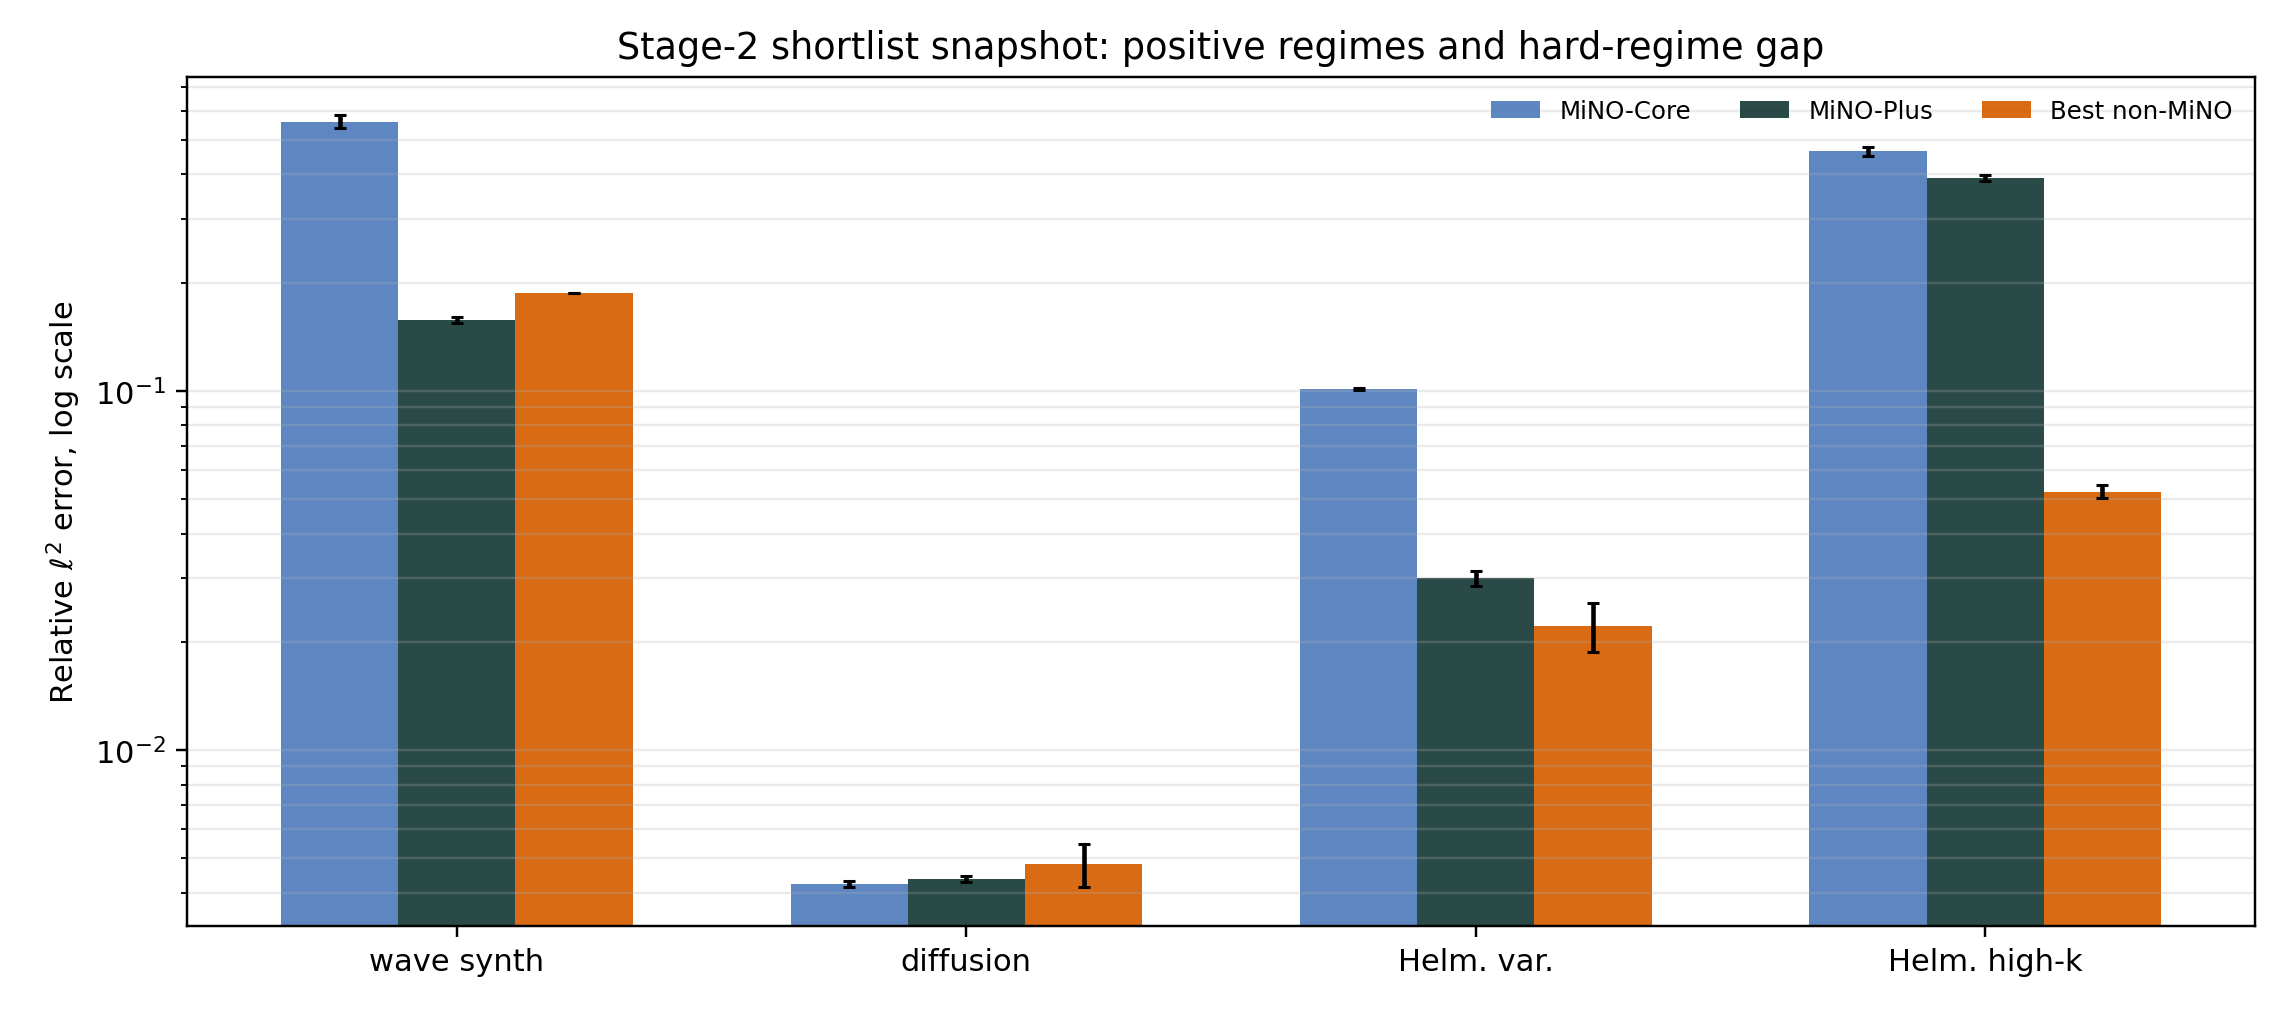
\includegraphics[width=0.96\textwidth]{figures/stage2_regime_snapshot.png}
\caption{Stage-2 shortlist snapshot.  The plot puts the positive rows and the high-$k$ Helmholtz motivation on the same log-scale axis.  \MiNO-Plus improves over \MiNO-Core on the wave and Helmholtz rows and is competitive on diffusion; the high-$k$ row motivates the branch/resolvent extension rather than serving as the main mechanism claim.}
\label{fig:stage2-regime-snapshot}
\end{figure}

\subsection{Branched High-\texorpdfstring{$k$}{k} Helmholtz Probe}
\label{sec:branched-helmholtz}

The high-$k$ Helmholtz row is the regime in which a single canonical graph is least plausible.  We therefore add a targeted finite-branch probe for Helmholtz.  The model uses $L=3$ independently parameterized canonical branches, token-wise metadata-softmax routing, branch entropy/diversity regularization, branch-summed transported synthesis and carrier paths, and the same admissible learned finite-landing layer used in the carrier-bound wave controls.  The default \MiNO\ model remains the $L=1$ carrier-bound architecture; the branched profile is used for the \texttt{helmholtz\_branched\_highk} campaign.

The executed rows are sample-capped and answer a narrow question: whether branch multiplicity alone is the active missing budget before adding the stronger outgoing resolvent-symbol layer.

The ablations are designed to separate finite-branch structure from ordinary transport use.  \texttt{single\_branch} forces the router onto branch 1 at fixed architecture, \texttt{no\_branch\_routing} replaces the learned router by uniform routing, \texttt{no\_transport} removes branch transport, \texttt{no\_transport\_no\_carrier} additionally removes transported synthesis/carrier/landing, and \texttt{no\_symbol} removes symbol modulation.  The criterion is conservative: a useful branch result should reduce the high-$k$ gap relative to the single-branch row, and otherwise the row is treated as a guide for the next microlocal budget rather than as a central claim.

The sample-capped branch-only result serves as a budget-local branch probe.  Across the three Helmholtz rows, the full $L=3$ branched model is close to the forced single-branch model, the uniform-routing ablation, and the no-symbol ablation.  This points to a sharper implementation requirement already predicted by the calculus ledger: branch multiplicity alone is too weak unless the frame, router, phase/landing, and outgoing resolvent-symbol budgets are all controlled.  The full table, routing plot, and field panels are kept in Appendix~\ref{app:diagnostic-figures}; the main text uses the row to motivate the \texttt{helmholtz\_resolvent} extension.

The follow-up \texttt{helmholtz\_highk\_careful} profile is therefore theory-aligned differently: it keeps the anisotropic packet frame and carrier-bound landing path, but replaces the generic \texttt{spectral\_order} multiplier by the executable \texttt{helmholtz\_resolvent} symbol layer from Corollary~\ref{cor:helmholtz-resolvent-symbol-budget}.  The layer uses an auto-calibrated shell and finite complex-pair multiplication for the signed outgoing resolvent factor, so the comparison is no longer merely an envelope-only symbol ablation.  Table~\ref{tab:helmholtz-highk-careful-midscale} reports the completed local mid-scale row and two matched profile checks.  Increasing the finite packet/resolvent capacity from the minimal smoke profile reduces the high-$k$ relative $\ell^2$ error from roughly $0.71$ to $0.50$.  The ablations also delimit the mechanism: forcing a single branch leaves the result unchanged, and removing the transport message alone is nearly flat, while removing both transport and the transported high-frequency carrier degrades strongly.  The \texttt{no\_symbol} row is close in relative $\ell^2$ and can be slightly better at some finite budgets, while its phase-sensitive diagnostics are worse; the matched \texttt{spectral\_order} row has essentially the same relative $\ell^2$ but worse phase than \texttt{helmholtz\_resolvent}.  The safe reading is therefore that the outgoing symbol layer is active and phase-sensitive, but is not yet a standalone relative-$\ell^2$ improvement.  The runner now separates this budget into \texttt{source\_only\_symbol}, \texttt{no\_edge\_symbol}, and \texttt{no\_resolvent\_phase} rows, with a small symbol-identity regularizer available when the local-kernel correction should remain a diagnostic rather than a default field-error path.  The matched \texttt{gabor\_gaussian} row has lower phase error but substantially worse relative $\ell^2$, so the high-$k$ field-error gain is attributed primarily to anisotropic packet resolution plus carrier-bound landing rather than to the isotropic Gabor frame.  Thus the current high-$k$ evidence supports anisotropic carrier-bound reconstruction more strongly than multibranch canonical transport, with the resolvent/local-kernel symbol remaining a phase/radiation budget under refinement.

\begin{table}[t]
\centering
\caption{Mid-scale \texttt{helmholtz\_highk\_careful} probe on \texttt{helmholtz\_highk\_positive}. Entries are three-seed means with standard deviations. The ablation block uses anisotropic packets, the \texttt{helmholtz\_resolvent} complex-pair symbol layer, two canonical branches, width 48, six modes, a transported landing decoder with eight channels, and 16 training epochs. The matched-profile block changes one calculus hook at a time. Lower is better.}
\label{tab:helmholtz-highk-careful-midscale}
\small
\begin{tabular}{lccc}
\toprule
Ablation & Rel. $\ell^2$ & Phase error & Imaginary resolvent energy \\
\midrule
\texttt{full} & $0.503\pm0.008$ & $1.511\pm0.028$ & $0.0349$ \\
\texttt{single\_branch} & $\mathbf{0.502}\pm0.005$ & $1.512\pm0.008$ & $0.0322$ \\
\texttt{no\_transport} & $0.506\pm0.011$ & $\mathbf{1.509}\pm0.006$ & $0.0229$ \\
\texttt{no\_transport\_no\_carrier} & $0.842\pm0.002$ & $1.499\pm0.015$ & $0.0424$ \\
\texttt{no\_symbol} & $0.509\pm0.012$ & $1.602\pm0.022$ & $0.0000$ \\
\bottomrule
\end{tabular}

\vspace{0.6em}
\begin{tabular}{lcc}
\toprule
Matched full-model profile & Rel. $\ell^2$ & Phase error \\
\midrule
\texttt{anisotropic\_gabor} + \texttt{helmholtz\_resolvent} & $0.503\pm0.008$ & $1.511\pm0.028$ \\
\texttt{anisotropic\_gabor} + \texttt{spectral\_order} & $\mathbf{0.502}\pm0.007$ & $1.609\pm0.037$ \\
\texttt{gabor\_gaussian} + \texttt{helmholtz\_resolvent} & $0.584\pm0.017$ & $\mathbf{1.486}\pm0.014$ \\
\bottomrule
\end{tabular}
\end{table}


\paragraph{Flagship high-frequency contract.}
The mid-scale row is not the full high-$k$ claim.  The registered flagship protocol is stricter: train on moderate frequencies, test on larger $k$, report nondimensional frequency $kL$, wavelengths across the domain, points per wavelength, reference-solver residual, complex relative $\ell^2$ when real/imaginary channels are present, amplitude and phase error, PDE residual, boundary/radiation residual, receiver or far-field trace error when available, runtime, memory, and error degradation as $k$ increases.  The runner now logs three finite proxies for this contract in addition to relative $\ell^2$: \texttt{test\_complex\_relative\_l2\_proxy}, which uses genuine real/imaginary channel pairs when the dataset supplies them; \texttt{test\_amplitude\_error\_proxy}, which measures envelope mismatch; and \texttt{test\_boundary\_trace\_error\_proxy}, which records a receiver-style boundary trace mismatch.  The baseline set is also tiered.  General neural operators (FNO, UNO/U-FNO, WNO, CNO/CANO-style attention when available) test whether the packet matrix improves over generic operator primitives.  Helmholtz-specialized solvers, including neural multigrid/Fourier and probabilistic high-frequency Helmholtz references, are required before claiming competitiveness in the high-$k$ solver literature.  The runner exposes this as \texttt{helmholtz\_highk\_flagship}; the campaign uses anisotropic packets, carrier-bound finite landing, \texttt{helmholtz\_resolvent}, OOD high-$k$ rows, and explicit complex-pair losses only when the dataset provides real/imaginary channels.  This protocol is the path from the current mechanism evidence to a high-$k$ flagship benchmark.

\subsection{Carrier-Bound Branch Identifiability}

The final \MiNO\ mechanism test is the carrier-bound \texttt{branch\_id\_v3} profile.  It keeps packet metadata batch-specific, uses Hamiltonian St\"ormer--Verlet metadata transport, synthesizes learned coefficients at transported packet centers, and adds a transported high-frequency input carrier from the original packet coefficients.  Skip and refinement paths are low-pass restricted, token-level refinement is disabled, and controlled-flow rows use the known packet drift as a metadata-flow target.  This makes transport a field-level mechanism: disabling transport leaves the high-frequency carrier at the analysis centers rather than the learned transported centers.

For fairness, the ablations are defined at the executable level.  \texttt{no\_transport} zeroes the propagation message and keeps identity metadata; it does not randomize packet centers.  \texttt{identity\_transport} keeps the propagation/message path but freezes displacement.  \texttt{randomized\_metadata} permutes metadata across packets, preserving the metadata multiset while breaking the packet--metadata association.  The same-refinement baseline column uses the same low-pass image-space refinement mechanism and training loss budget as \MiNO-Plus, but without MiNO's packet tokenizer, transported synthesis, transported carrier, or token-level packet refinement.  The registered \texttt{branch\_id\_v3\_controls} campaign adds two fairness controls: \texttt{full\_no\_flow\_supervision}, which removes metadata-flow supervision at fixed architecture, and \texttt{no\_transport\_no\_carrier}, which removes both transport and the transported high-frequency carrier.  These controls separate flow-supervision dependence, carrier binding, and learned transport corruption.

\begin{table}[t]
\centering
\caption{Carrier-bound \texttt{branch\_id\_v3} mechanism test. Entries are mean relative $\ell^2$ over three seeds; lower is better. Scenario aliases match the five controlled wave rows listed in the text.}
\label{tab:branchidv3}
\small
\scriptsize
\begin{tabular}{@{}p{0.16\textwidth}ccccc@{}}
\toprule
Scenario & \MiNO & No transport & Random metadata & No symbol & Best same-refine \\
\midrule
bichar. & 0.380 & 0.714 & 0.912 & 0.395 & 0.056 (UNO) \\
chirp & 0.316 & 0.839 & 1.048 & 0.335 & 0.070 (UNO) \\
two-packet & 0.204 & 0.777 & 1.037 & 0.236 & 0.022 (UNO) \\
var-speed & 0.239 & 0.456 & 0.890 & 0.240 & 0.074 (UNO) \\
wave synth & 0.295 & 0.537 & 0.900 & 0.298 & 0.154 (UNO) \\
\bottomrule
\end{tabular}
\end{table}

The controls table below is generated from the completed \texttt{branch\_id\_v3\_controls} summary.  It is the fairness counterpart to Table~\ref{tab:branchidv3}: \texttt{full\_no\_flow\_supervision} tests whether the effect is merely flow-supervision driven, and \texttt{no\_transport\_no\_carrier} tests whether the degradation is explained by the transported carrier path alone.  Across all five rows, removing flow supervision changes relative $\ell^2$ by at most $0.020$, while removing transport increases relative $\ell^2$ by $0.217$--$0.574$.  Removing both transport and the high-frequency carrier remains worse than the full model in every row, and is worse than \texttt{no\_transport} in four of the five rows.

\begin{table}[t]
\centering
\caption{Registered \texttt{branch\_id\_v3\_controls} field-error checks. Entries are mean relative $\ell^2$ over three seeds; lower is better.}
\label{tab:branchidv3controls}
\scriptsize
\begin{tabular}{lccccccc}
\toprule
Scenario & Full & No flow & No tr. & Identity & No tr./car. & Rand. meta & No sym. \\
\midrule
bichar. & 0.378 & 0.379 & 0.715 & 0.714 & 0.815 & 0.912 & 0.392 \\
chirp & 0.315 & 0.319 & 0.840 & 0.806 & 0.826 & 1.044 & 0.334 \\
two-packet & 0.205 & 0.185 & 0.779 & 0.749 & 0.801 & 1.038 & 0.234 \\
var-speed & 0.238 & 0.238 & 0.455 & 0.456 & 0.753 & 0.892 & 0.240 \\
wave synth & 0.296 & 0.296 & 0.534 & 0.535 & 0.774 & 0.905 & 0.298 \\
\bottomrule
\end{tabular}
\end{table}


The ablation pattern is coherent.  Removing transport increases field error in every row; identity transport behaves like the transport-off control; randomizing metadata increases the error further; removing only the symbol branch has a smaller effect on these transport-dominant wave probes.  The same-refinement baselines are included as absolute-accuracy controls.  Tables~\ref{tab:branchidv3}--\ref{tab:branchidv3controls} therefore establish the main empirical point: the final \MiNO\ architecture uses packet transport as a causal field-level branch under the registered carrier-bound protocol.

\begin{table}[t]
\centering
\caption{Theorem-to-metric map for the carrier-bound mechanism evidence.  The table records what each theorem budget predicts experimentally and which registered row probes it.}
\label{tab:theorem-metric-map}
\scriptsize
\begin{tabular}{p{0.22\textwidth}p{0.27\textwidth}p{0.27\textwidth}p{0.13\textwidth}}
\toprule
Theorem term & Artifact metric & Registered probe & Status \\
\midrule
Transport budget $E_{\mathrm{tr}}$ & relative $\ell^2$, canonical-flow proxy, WF-transport proxy & \texttt{no\_transport}, \texttt{identity\_transport}, \texttt{randomized\_metadata} & tested \\
Transported synthesis $E_{\mathrm{tsyn}}$ & field error under transported synthesis corruption & \texttt{identity\_transport} vs full & tested \\
Carrier channel $E_{\mathrm{car}}$ & extra degradation after removing transported carrier & \texttt{no\_transport\_no\_carrier} vs \texttt{no\_transport} & tested \\
Symbol budget $E_{\mathrm{sym}}$ & relative $\ell^2$, symbol-order proxy & \texttt{no\_symbol} & tested \\
Packet tail $E_{\mathrm{tail}}$ & packet-WF localization and future $K$ sweep & fixed-$K$ controls; budget sweep deferred & partial \\
Frame/asymptotic/covering $E_{\mathrm{frame}},E_{\mathrm{asymp}},\delta_h$ & tokenizer reconstruction, frame diagnostics, resolution sweep & cross-resolution campaign & deferred \\
\bottomrule
\end{tabular}
\end{table}

This table also fixes the interpretation of the mechanism claim.  Field degradation under transport corruption is a causal-use test.  On controlled rows we additionally log canonical-flow and packet-wavefront proxies; budget-scaling in $K$, transport capacity, symbol capacity, and packet resolution is the natural quantitative follow-up.

\paragraph{Executable landing diagnostic.}
The theory idealizes a packet synthesis operator with controlled frame constants, while the executable model must land transported packet content on a finite pixel grid.  We therefore ran a synthesis-mode probe on the two cleanest wavefront scenarios.  Two analytic replacements for the packet-energy warp, moved Gabor-atom splatting and moved local-patch folding, were substantially worse.  A transport-conditioned finite landing decoder was the only tested landing map that reduced the UNO gap in the single-seed diagnostic, reaching relative $\ell^2$ $0.056$ on \texttt{wave\_chirp\_propagation} and $0.034$ on \texttt{wave\_two\_packet\_no\_interaction}.  The narrow theoretical reading is that the learned decoder reduces the executable landing terms $E_{\mathrm{tsyn}}$ and $E_{\mathrm{car}}$; it does not change the canonical propagation theorem and it is not a new microlocal calculus result.

\begin{table}[t]
\centering
\caption{Single-seed executable landing probe.  This table is diagnostic, not a replacement for the registered three-seed mechanism tables.  It tests whether the remaining UNO gap is partly a finite landing problem rather than a canonical-flow problem.}
\label{tab:synthesis-mode-probe}
\small
\begin{tabular}{p{0.23\textwidth}p{0.18\textwidth}ccc}
\toprule
Scenario & Landing map & Full & No transport & UNO+ref \\
\midrule
chirp & warp & 0.316 & 0.839 & 0.070 \\
 & atom splat & 0.801 & 0.841 & 0.048 \\
 & patch fold & 0.758 & 0.662 & 0.047 \\
 & learned landing & 0.056 & 0.093 & 0.048 \\
\addlinespace
two-packet & warp & 0.204 & 0.777 & 0.022 \\
 & atom splat & 0.680 & 0.836 & 0.021 \\
 & patch fold & 0.764 & 0.743 & 0.022 \\
 & learned landing & 0.034 & 0.053 & 0.022 \\
\bottomrule
\end{tabular}
\end{table}


\begin{figure}[t]
\centering
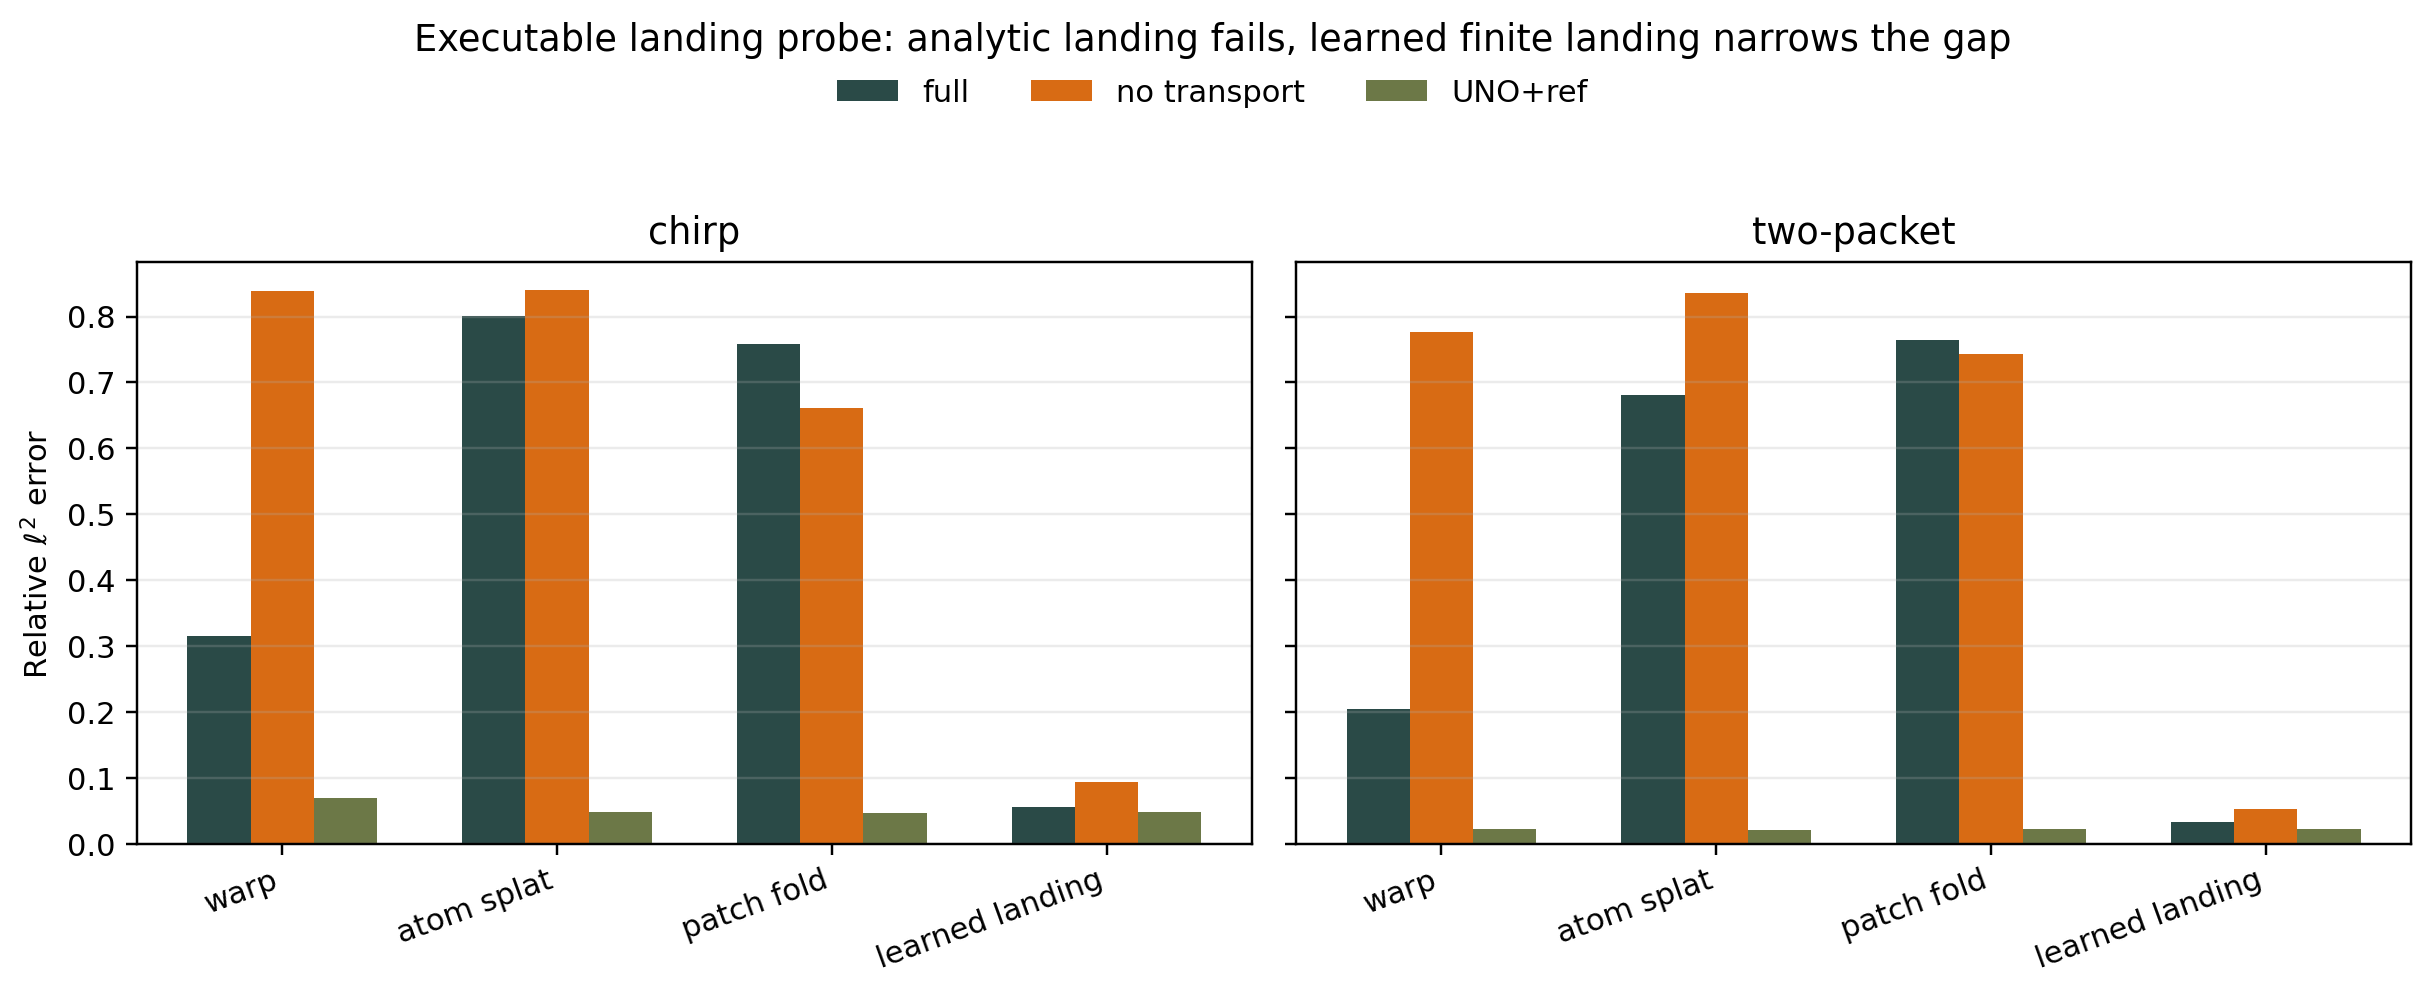
\includegraphics[width=\textwidth]{figures/synthesis_mode_probe_relative_l2.png}
\caption{Single-seed executable landing probe.  The instability of analytic atom-splat and moved-patch folding indicates that the UNO gap is partly an executable finite-landing problem.  The learned landing decoder narrows this gap while preserving a transport ablation penalty, so it is treated as a finite landing layer for $E_{\mathrm{tsyn}}$ and $E_{\mathrm{car}}$.}
\label{fig:synthesis-mode-probe}
\end{figure}

We then promoted the learned finite-landing row to a three-seed \texttt{branch\_id\_v3\_controls} follow-up.  Table~\ref{tab:learned-landing-controls} and Figure~\ref{fig:learned-landing-controls} show the outcome.  The learned landing layer sharply improves absolute field error relative to the analytic finite-landing controls, but it does not erase the transport mechanism: \texttt{no\_transport} remains worse than \texttt{full} in every row, and removing both transport and the high-frequency carrier remains much worse.  The effect is smaller than in the non-decoder carrier-bound table, so the decoder is treated as a finite implementation layer that reduces landing error while preserving a residual transport penalty.  The \texttt{no\_symbol} rows remain flat or slightly better in several scenarios; these learned-landing controls therefore strengthen finite-landing evidence, not symbol-branch attribution.

\begin{table}[t]
\centering
\caption{Three-seed learned finite-landing controls.  Entries are mean relative $\ell^2$; lower is better.  The transport-conditioned decoder reduces absolute field error relative to the analytic finite-landing maps, while transport removal and carrier removal remain visible.}
\label{tab:learned-landing-controls}
\scriptsize
\begin{tabular}{lcccccc}
\toprule
Scenario & Full & No flow & No tr. & No tr./car. & Rand. meta & No sym. \\
\midrule
bichar. & 0.060 & 0.059 & 0.090 & 0.814 & 0.722 & 0.050 \\
chirp & 0.057 & 0.067 & 0.104 & 0.862 & 0.845 & 0.053 \\
two-packet & 0.036 & 0.051 & 0.050 & 0.828 & 0.888 & 0.031 \\
var-speed & 0.072 & 0.086 & 0.144 & 0.754 & 0.752 & 0.101 \\
wave synth & 0.179 & 0.180 & 0.219 & 0.771 & 0.779 & 0.178 \\
\bottomrule
\end{tabular}
\end{table}


\begin{figure}[t]
\centering
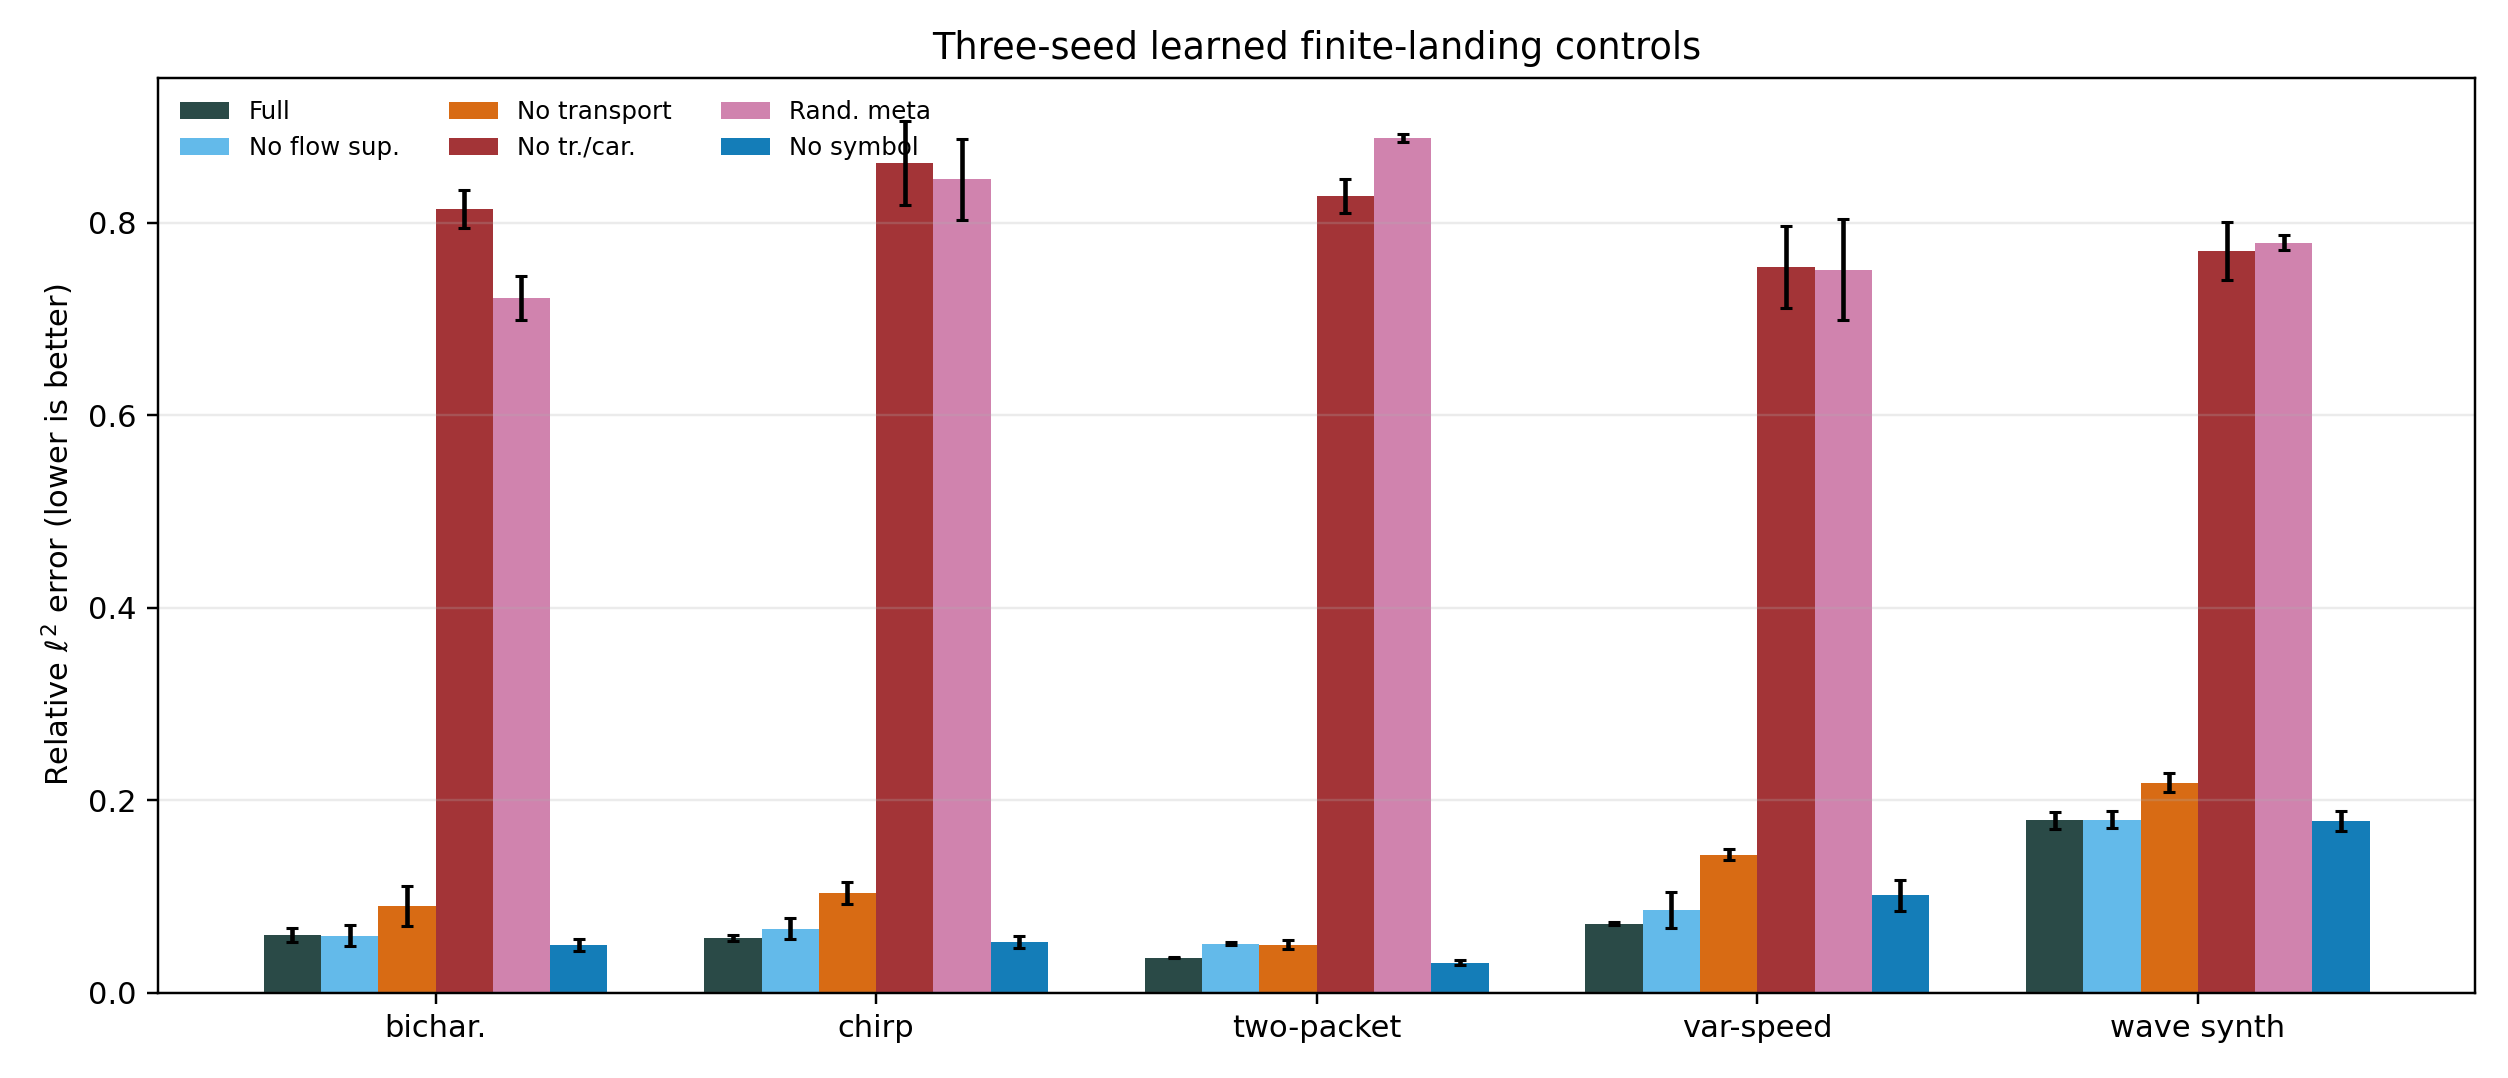
\includegraphics[width=\textwidth]{figures/learned_landing_controls_relative_l2.png}
\caption{Three-seed learned finite-landing controls.  The transport-conditioned decoder reduces absolute field error on controlled wave probes, while \texttt{no\_transport}, \texttt{no\_transport\_no\_carrier}, and metadata randomization remain degraded.  The result supports a finite landing correction that preserves transport dependence.}
\label{fig:learned-landing-controls}
\end{figure}

\begin{figure}[t]
\centering
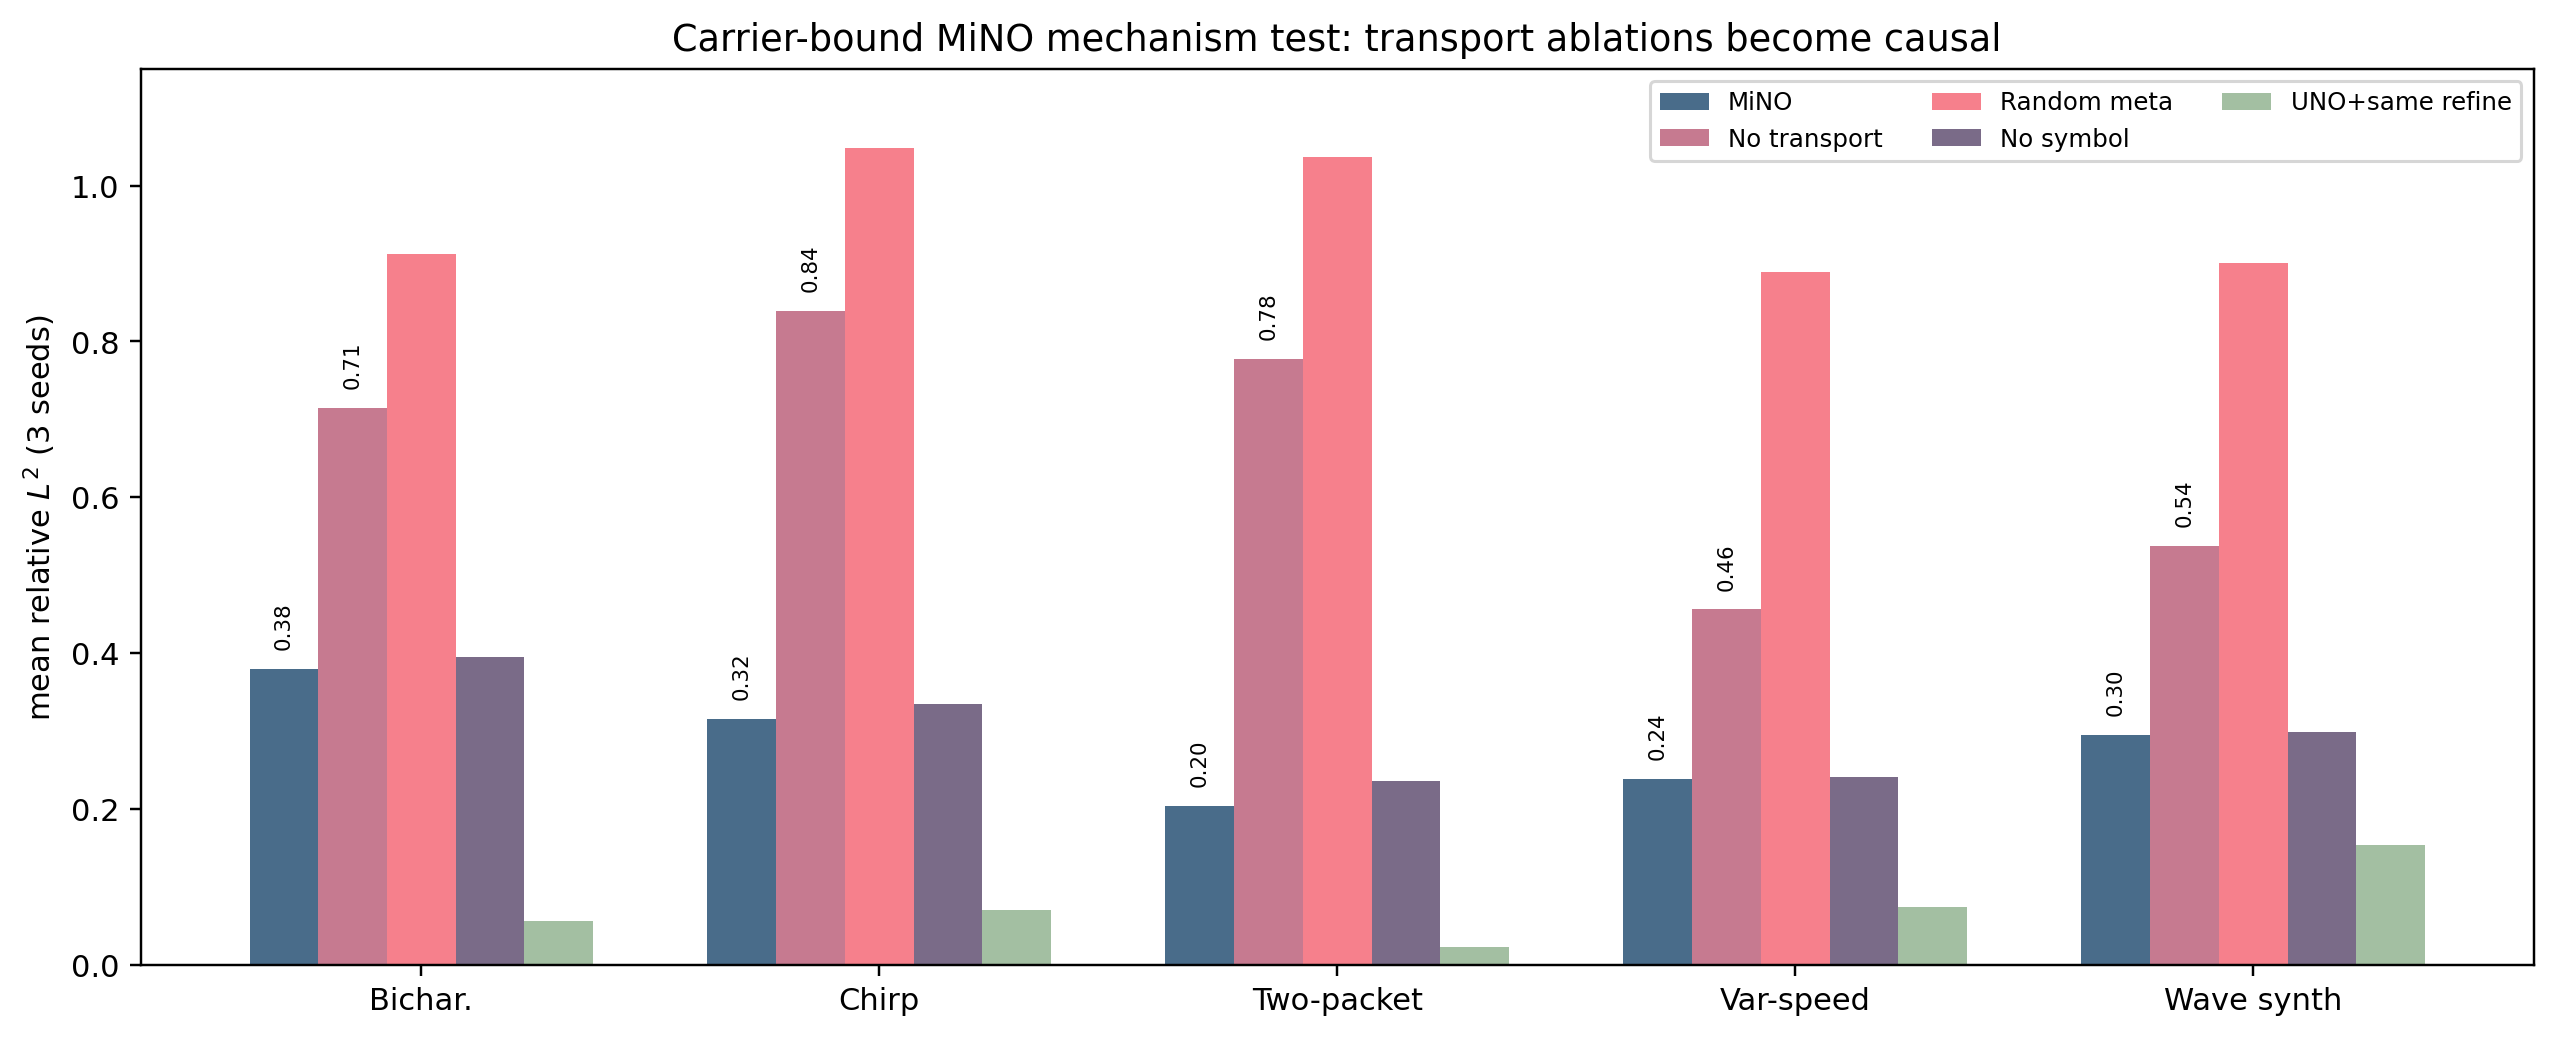
\includegraphics[width=\textwidth]{figures/branch_id_v3_carrier_mechanism_bars.png}
\caption{Carrier-bound branch-identifiability results.  Transport removal and metadata randomization produce a consistent degradation pattern across controlled wave probes, while same-refinement baselines remain a separate absolute-accuracy control.}
\label{fig:branch-id-v3-carrier-bars}
\end{figure}

\begin{figure}[t]
\centering
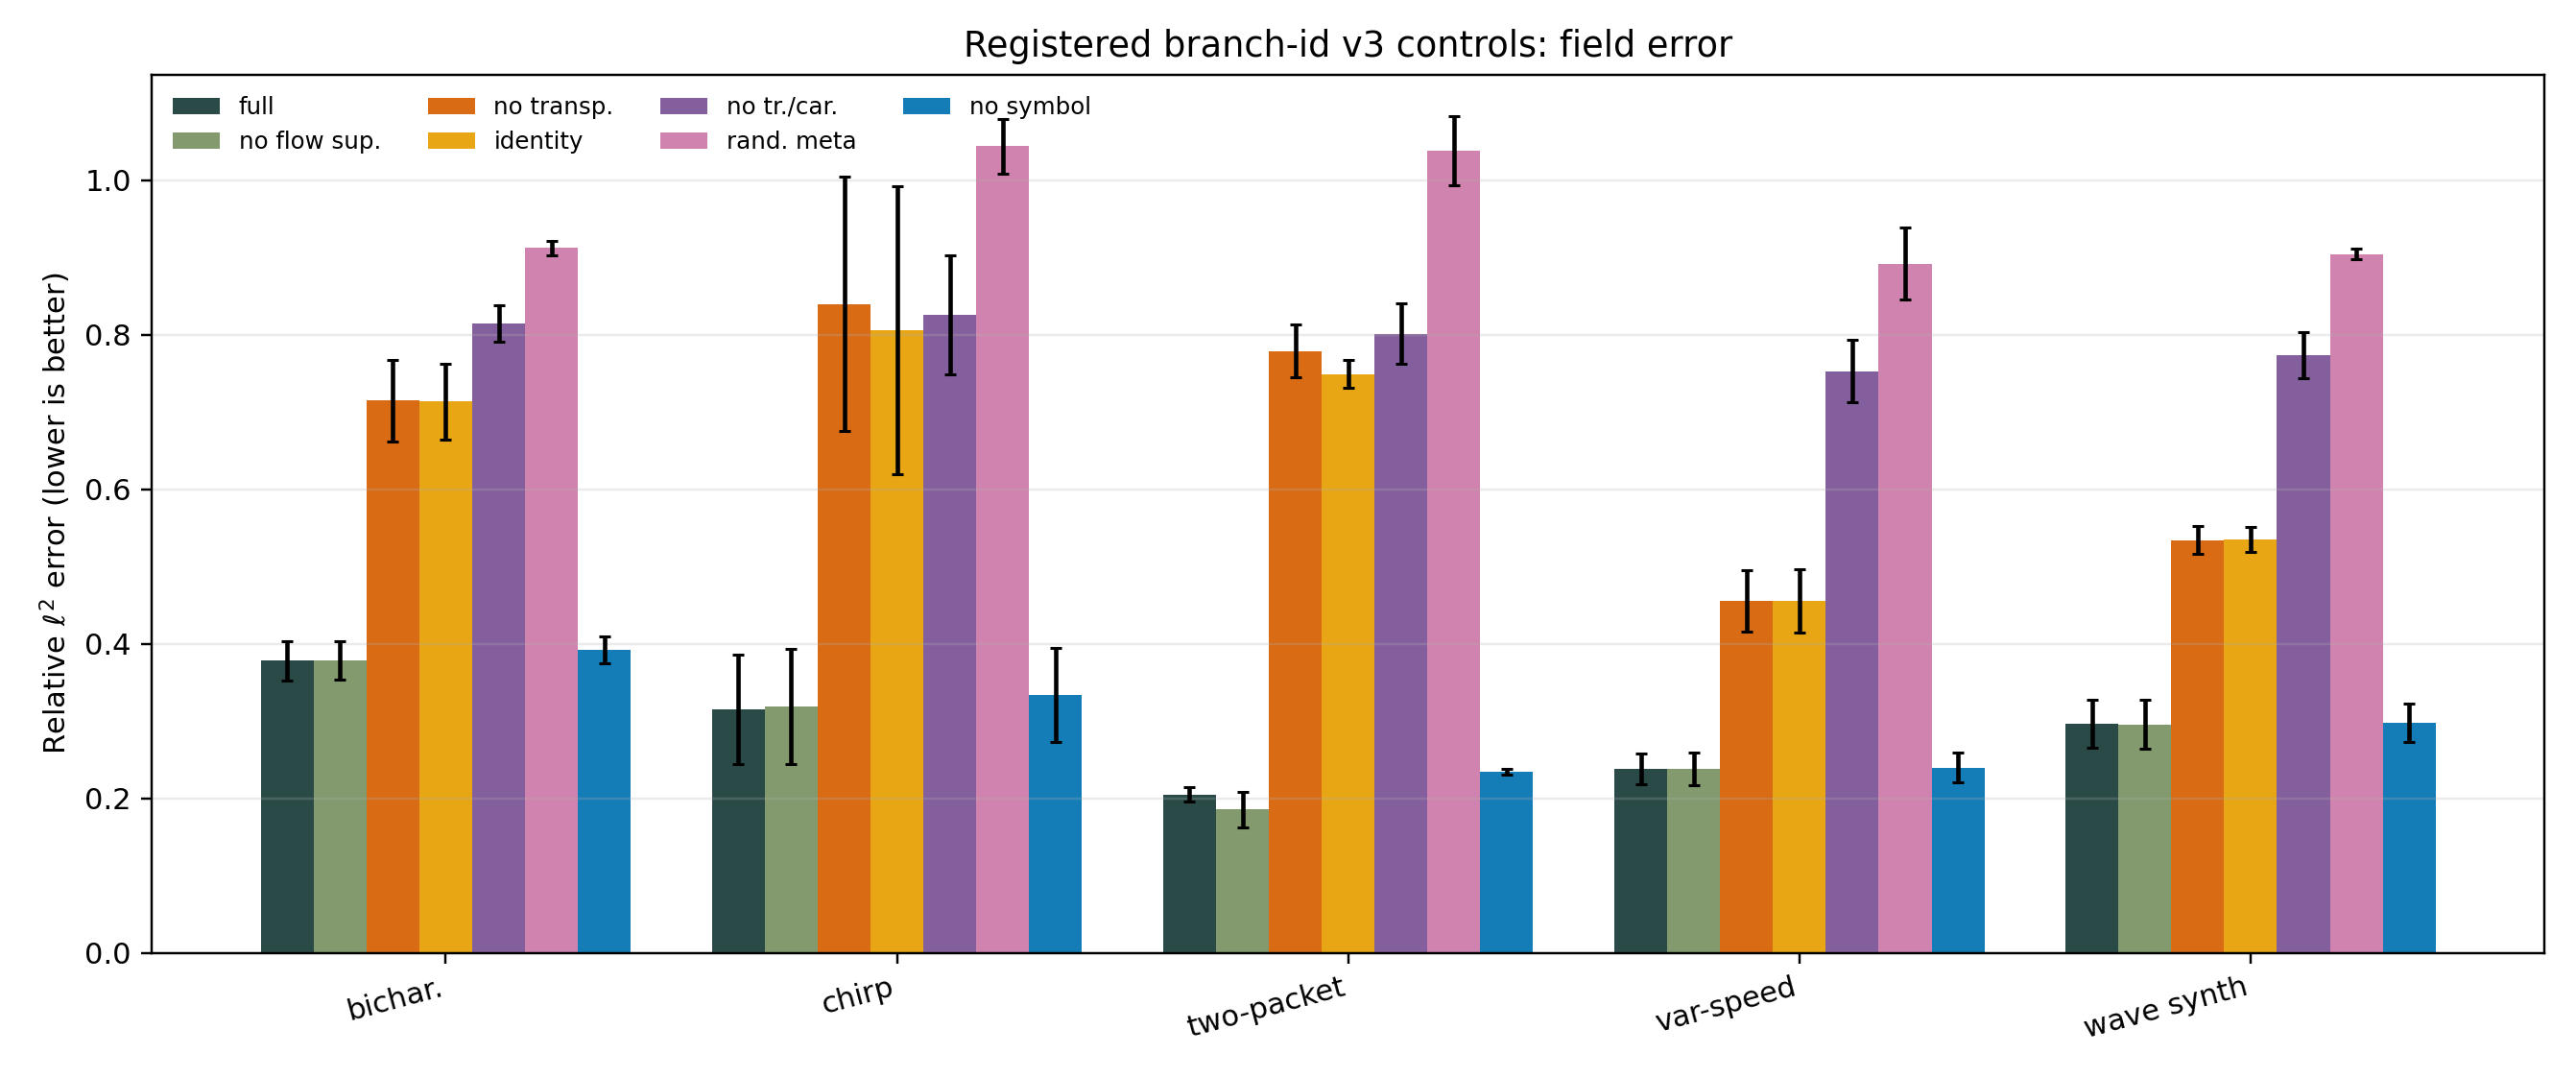
\includegraphics[width=\textwidth]{figures/branch_id_v3_controls_relative_l2.png}
\caption{Registered \texttt{branch\_id\_v3\_controls} field-error checks.  The key comparisons are \texttt{full\_no\_flow\_supervision} versus \texttt{full}, and \texttt{no\_transport\_no\_carrier} versus \texttt{no\_transport}.  Flow supervision is not needed for the reported field-error effect, while carrier removal separates the high-frequency carrier contribution from the transport-corruption contribution.}
\label{fig:branch-id-v3-controls-l2}
\end{figure}

\begin{figure}[t]
\centering
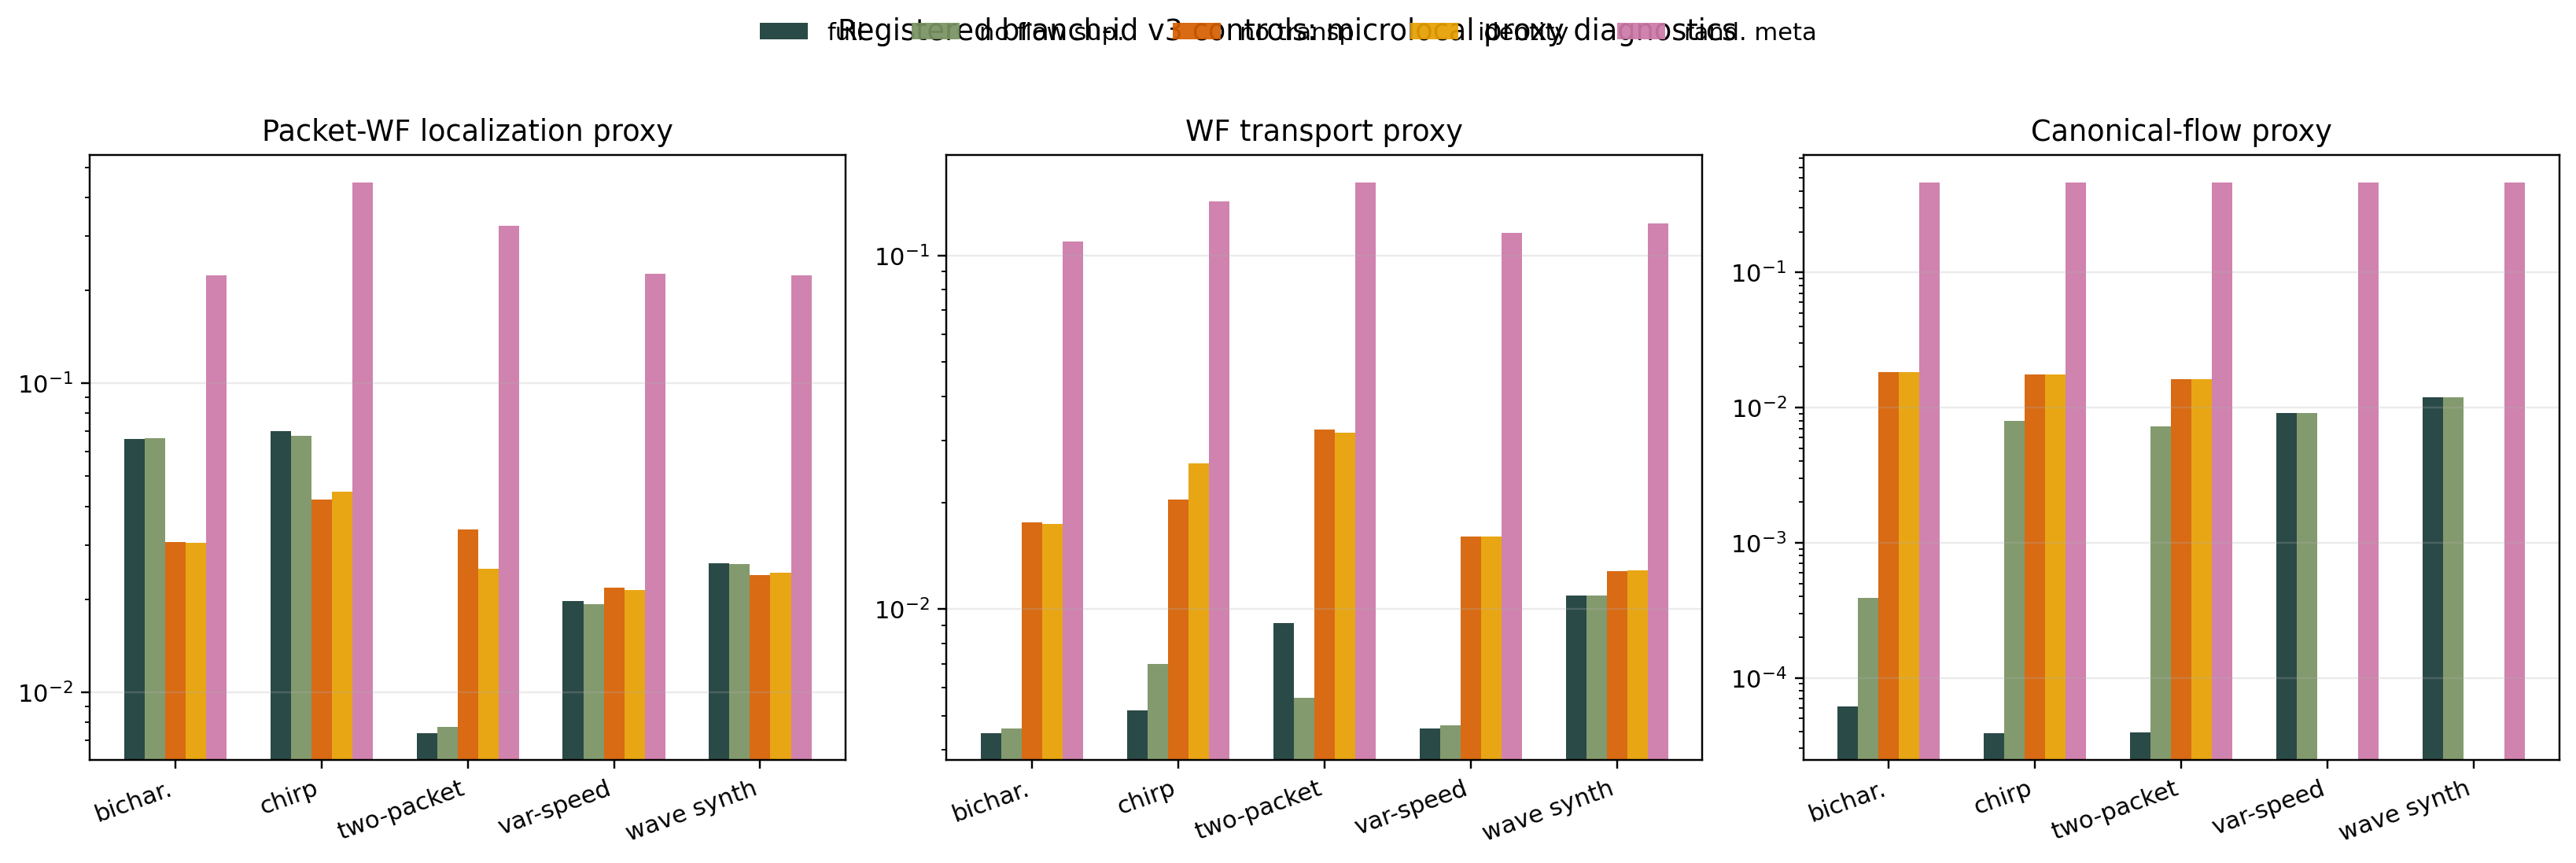
\includegraphics[width=\textwidth]{figures/branch_id_v3_controls_wavefront_proxy.png}
\caption{Registered \texttt{branch\_id\_v3\_controls} microlocal-proxy checks.  The plotted diagnostics correspond to Corollary~\ref{cor:packet-wavefront-localization}: packet-wavefront localization error, wavefront-transport proxy error, and canonical-flow proxy error.  These are mechanism diagnostics rather than aggregate SOTA metrics.}
\label{fig:branch-id-v3-controls-wf}
\end{figure}

\begin{figure}[t]
\centering
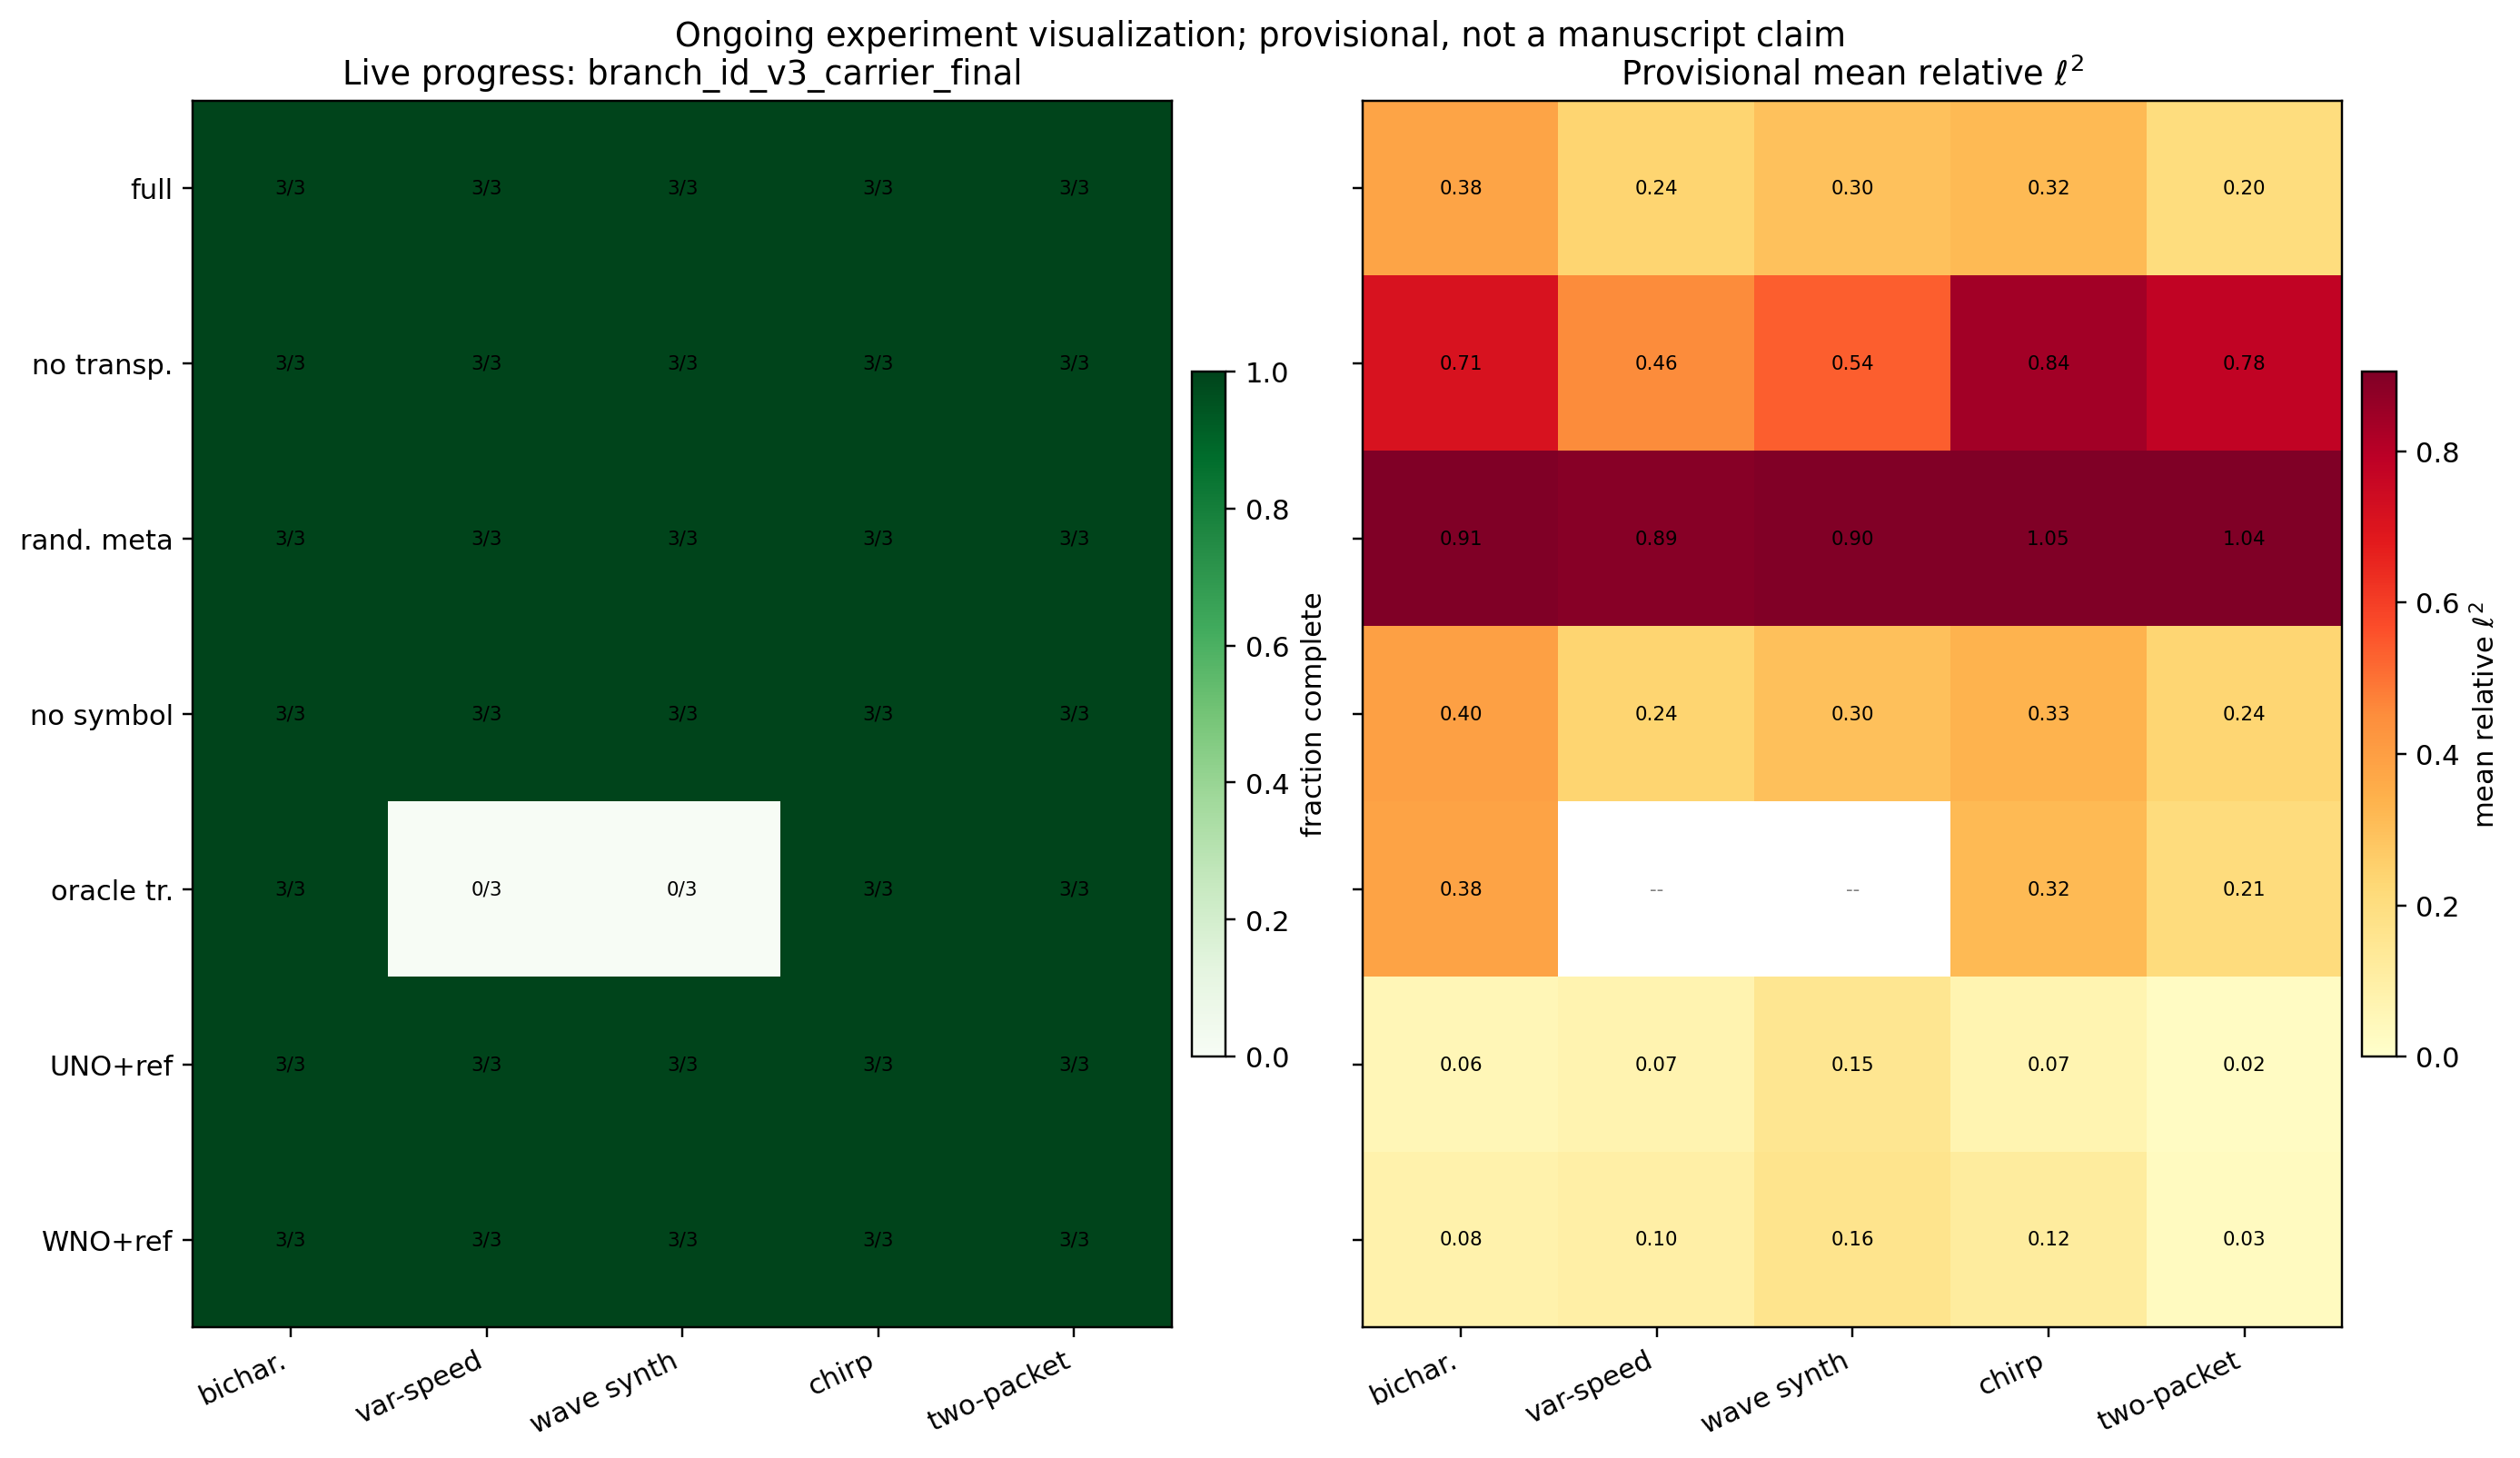
\includegraphics[width=0.92\linewidth]{figures/branch_id_v3_carrier_final_live.png}
\caption{Completed \texttt{branch\_id\_v3} campaign matrix generated by the resumable runner.  Each cell records the completed seed count and the mean relative $\ell^2$ used to build Table~\ref{tab:branchidv3}.}
\label{fig:branch-id-v3-carrier-live}
\end{figure}

\subsection{Claim Matrix}

\begin{table}[t]
\centering
\caption{Claim-to-regime matrix for the carrier-bound \MiNO\ manuscript.}
\label{tab:claimmatrix}
\small
\begin{tabular}{p{0.30\textwidth}p{0.24\textwidth}p{0.32\textwidth}}
\toprule
Claim & Evidence & Verdict \\
\midrule
\MiNO-Core is a theorem-facing packet architecture & $\ell^2$ packet-matrix theorem plus finite Lean landing layer and executable Core model & supported \\
Carrier-bound \MiNO\ makes transport field-causal & branch-ID ablations and controls & supported on controlled wave probes \\
Learned finite landing reduces executable synthesis error & learned-landing controls & supported as finite implementation evidence; transport penalty remains \\
Symbol branch is the dominant wave mechanism & \texttt{no\_symbol} rows & not the dominant effect on these transport-dominant probes \\
Identity/dissipative packet regimes are useful & diffusion rows near strongest imported references & supported as aggregate performance; symbol-branch attribution still requires calculus-regime ablations \\
High-$k$ Helmholtz is a stress diagnostic for anisotropic carrier-bound reconstruction & Table~\ref{tab:helmholtz-highk-careful-midscale} and Corollary~\ref{cor:helmholtz-resolvent-symbol-budget} & local mid-scale improvement; anisotropic packets and carrier-bound landing drive the field-error gain, the resolvent/local-kernel symbol is phase-sensitive but not field-error-positive at every budget, and branch multiplicity is not identified in this row \\
Local-window Helmholtz/Navier probes delimit extension regimes & local-window Helmholtz and synthetic Navier calculus probes & scoping diagnostics for branch/resolvent and transport--diffusion profiles \\
\bottomrule
\end{tabular}
\end{table}

The low-budget local-window Helmholtz and synthetic Navier--Stokes panels are kept as appendix diagnostics (Figures~\ref{fig:helmholtz-navier-calculus-probe}--\ref{fig:helmholtz-navier-prediction-panels}).  They delimit extension regimes and are not part of the main positive evidence.

\subsection{Interpretation}

The empirical evidence aligns with two mechanism statements.  On controlled wave probes, the carrier-bound model makes transported metadata field-causal: transport corruption degrades field error after low-frequency residual paths are restricted.  On the high-$k$ Helmholtz row, the active mechanism is different: the robust field-error signal is carried by anisotropic packet resolution, the transported high-frequency carrier, and finite landing.  The high-$k$ mid-scale ablation does not identify multibranch canonical transport, since \texttt{single\_branch} and \texttt{no\_transport} are essentially flat against \texttt{full}.  The matched profile checks separate the calculus terms: replacing the resolvent/local-kernel symbol changes phase-sensitive behavior more than relative $\ell^2$, while replacing anisotropic packets by isotropic Gabor packets worsens field error.
